\documentclass{report}
\usepackage[fontsize=13pt]{scrextend}

\usepackage{my_lab}

\begin{document}

\MiptLabTitle{4.3.1}{ИЗУЧЕНИЕ ДИФРАКЦИИ СВЕТА}

\begin{document}
\textbf{Цель работы}: исследовать являения дифракции Френеля и Фраунгофера на
щели, изучить влияние дифракции на разрешающую способность оптических
инструментов.

\textbf{В работе используются}: оптическая скамья, ртутная лампа, монохроматор,
щели с регулируемой шириной, рамка с вертикальной нитью, двойная щель,
микроскоп на поперечных салазках с микрометрическим винтом, зрительная труба.

\section*{Установка}
\begin{figure}[H]
	\centering
	\includegraphics[width=0.9\linewidth]{figures/schema-А.png}
	\caption{Схема установки для наблюдения дифракции Френеля}
\end{figure}
\begin{description}
	\item[М] -- микроскоп.
	\item[П] -- плоскость фокуса микроскопа.
	\item[$O_1$] -- линза с ф.р. $f_1$.
	\item[Л] -- лампа.
	\item[С] -- монохроматор.
	\item[$S_1, S_2$] -- щели.
\end{description}

Суммарная ширина m зон Френеля:
\begin{equation}
	z_m = \sqrt{a m \lambda}
\end{equation}

Число Френеля:
\begin{equation}
	\Phi^2 = \dfrac{D}{\sqrt{a \lambda}}
\end{equation}

Волновой параметр:
\begin{equation}
	p = \frac{1}{\Phi^2}
\end{equation}

\section*{А. Дифракция Френеля}

Условие наблюдения дифракции:
\begin{equation}
	\Phi \gtrsim 1
\end{equation}

Пусть $m$ -- число зон Френеля, укладывающихся на полуширине щели,\\
тогда будет видно $n = m - 1$ темных полос.

\section*{Б. Дифракция Фраунгофера на щели}

\begin{equation}
	\Phi \ll 1
\end{equation}

\begin{figure}[H]
	\centering
	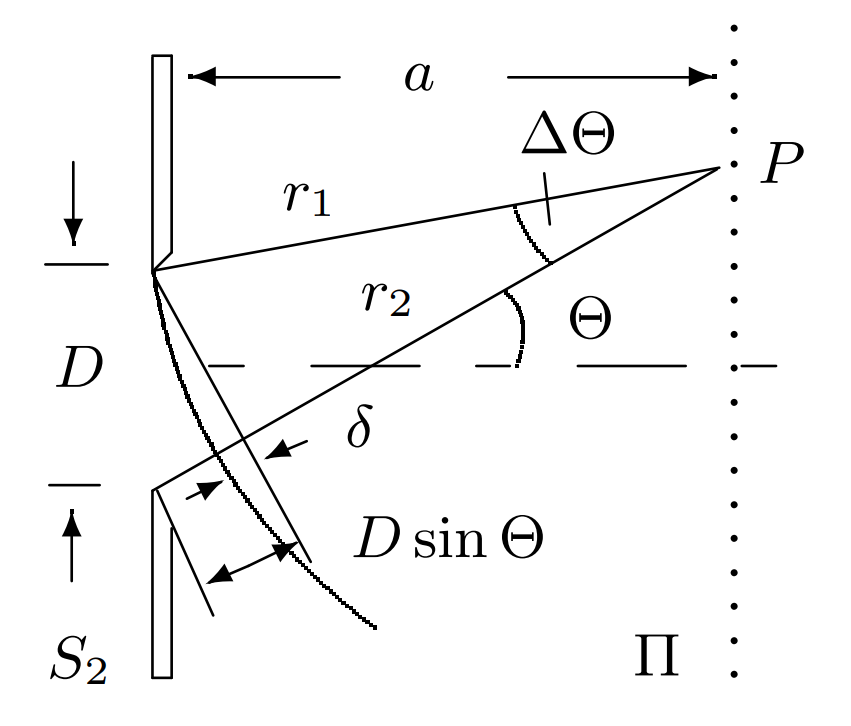
\includegraphics[width=0.5\linewidth]{figures/дифракция_Фраунгофера.png}
	\caption{К фазовым соотношениям при дифракции Фраунгофера}
\end{figure}

\begin{equation}
	\Delta \approx D \theta
\end{equation}

\begin{figure}[H]
	\centering
	\includegraphics[width=0.9\linewidth]{figures/schema-Б.png}
	\caption{Схема установки для наблюдения дифракции Фраунгофера на щели}
\end{figure}

К схеме A добавляется линза $O_2$ с фокусным расстоянием $f_2$.

\begin{figure}[H]
	\centering
	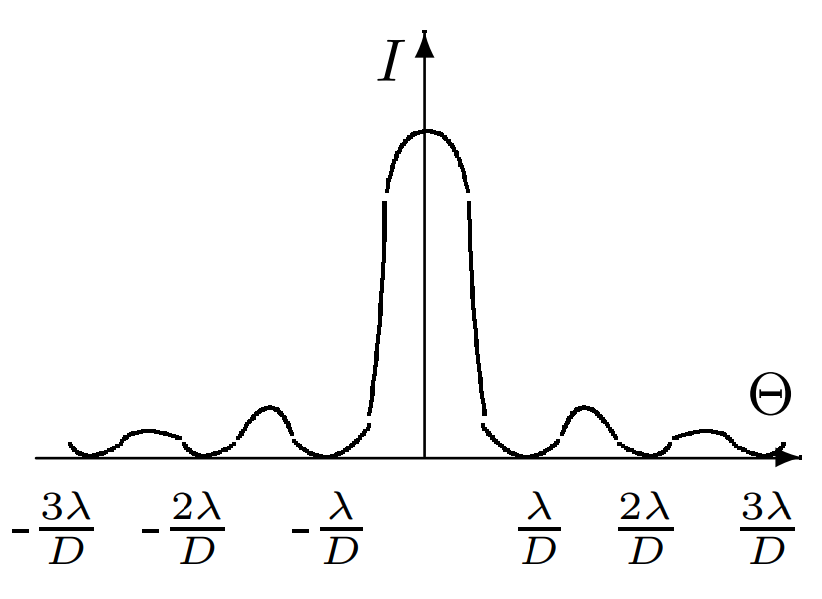
\includegraphics[width=0.6\linewidth]{figures/распр.png}
	\caption{Распределение интенсивности при дифракции Фраунгофера на
		щели}
\end{figure}

\begin{equation}
    X \approx f_2 \theta
\end{equation}

Положения темных полос:
\begin{equation}
    \theta_m = \frac{m \lambda}{D}, \quad m \in \NN
\end{equation}
\begin{equation}
    X_m \approx m \frac{f_2 \lambda}{D}
\end{equation}

\section*{В. Дифракция Фраунгофера на двух щелях}

\begin{figure}[H]
    \centering
    \includegraphics[width=0.9\linewidth]{figures/schema-В.png}
\end{figure}

От схемы Б. \\
$S_2$ заменяем на экран \textbf{Э} с двумя щелями.

Положения темных полос:
\begin{equation}
    \theta_m = m \frac{\lambda}{d}
\end{equation}
\begin{equation}
    X_m = m \frac{\lambda f_2}{d}
\end{equation}
\begin{equation}
    \delta X = \frac{\lambda f_2}{d}
\end{equation}

Кол-во полос в главном максимуме:
\begin{equation}
    n = \frac{2 \lambda f_2}{D} \frac{1}{\delta X} = 2 \frac{d}{D}
\end{equation}

Условие наблюдения дифракции:
\begin{equation}
    b \le f_1 \frac{\lambda}{d}
\end{equation}
$b$ -- ширина входной щели S.

\section*{Г. Влияние дифракции на разрешающую способность оптического
инструмента}

\begin{figure}[H]
    \centering
    \includegraphics[width=0.9\linewidth]{figures/schema-Г.png}
    \caption{Схема установки для исследования разрешающей способности
    оптического инструмента}
\end{figure}

От схемы Б. \\
$S_1$ заменяем на экран \textbf{Э} с двумя щелями.

\begin{equation}
    \varphi = \frac{d}{f_1}
\end{equation}
\begin{equation}
    l = \varphi f_2 = d \frac{f_2}{f_1}
\end{equation}

\begin{figure}[H]
    \centering
    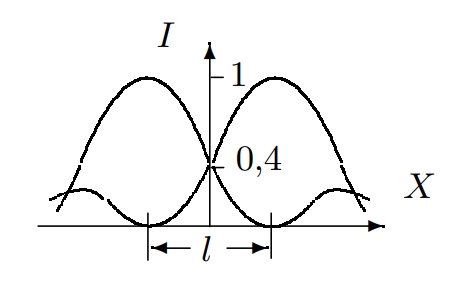
\includegraphics[width=0.6\linewidth]{figures/критерий_Рэлея.png}
    \caption{Критерий разрешения по Рэлею}
\end{figure}
\begin{equation}
    \varphi = \frac{\lambda}{D_0} = \frac{l}{f_2} = \frac{d}{f_1}
\end{equation}

\section*{Теоретическая часть}

\section*{Ход работы}

\section*{Выводы}

\end{document}
